% This text is proprietary.
% It's a part of presentation made by myself.
% It may not used commercial.
% The noncommercial use such as private and study is free
% Dec 2007
% Author: Sascha Frank 
% University Freiburg 
% www.informatik.uni-freiburg.de/~frank/
%
% 
\documentclass{beamer}
\usepackage[utf8]{inputenc}
\usepackage[english]{babel}
\usepackage{amsmath}
\usepackage{amsfonts}
\usepackage{amssymb}
\usepackage{graphicx}
\usepackage{empheq}
\usepackage{mathrsfs}
%
%\usepackage[listings,theorems]{tcolorbox}

\setbeamertemplate{navigation symbols}{}

\setbeamercolor{frametitle}{fg=black,bg=white}
\setbeamercolor{title}{fg=black,bg=white!85!blue}
%\usetheme{Boadilla}
\usetheme{Szeged}


\makeatletter
    \newenvironment{withoutheadline}{
        \setbeamertemplate{headline}[default]
        \def\beamer@entrycode{\vspace*{-\headheight}}
    }{}
\makeatother

\beamersetuncovermixins{\opaqueness<1>{25}}{\opaqueness<2->{15}}
\begin{document}

%==============================================================
\author[]{H. Aghakhani}
\title{Paper review: Statistical analysis and
simulation of random shocks
in stochastic Burgers equation}
\institute{MTH 837}
%==============================================================
\frame{\titlepage} 
\frame{\frametitle{Table of contents}\tableofcontents} 
%==============================================================
\begin{withoutheadline}

\begin{frame} \frametitle{Title and Authors}

\includegraphics[width=\textwidth]{1.png} 

\end{frame}
\end{withoutheadline}
%==============================================================
\section{Motivation}
\begin{withoutheadline}

\begin{frame} \frametitle{Motivation}
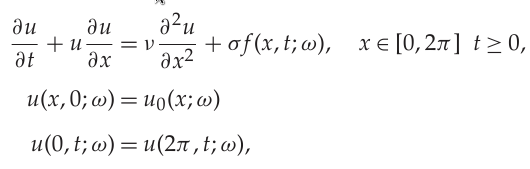
\includegraphics[width=.8\textwidth]{3.png}
\begin{itemize}
\item Burger's equation is a very important equation, and is used as a case study for for variety of different stochastic methods.
\item It has nonlinear term (advection term)
\item It has a laplacian term (diffusion term)
\item it has source term
\item Depend on which term is dominant this equation could have different behavior. 
\item It can be considered as simple 1D Navier\_Stockes equations
\end{itemize}
\end{frame}
\end{withoutheadline}
%==============================================================
\begin{withoutheadline}

\begin{frame} \frametitle{}
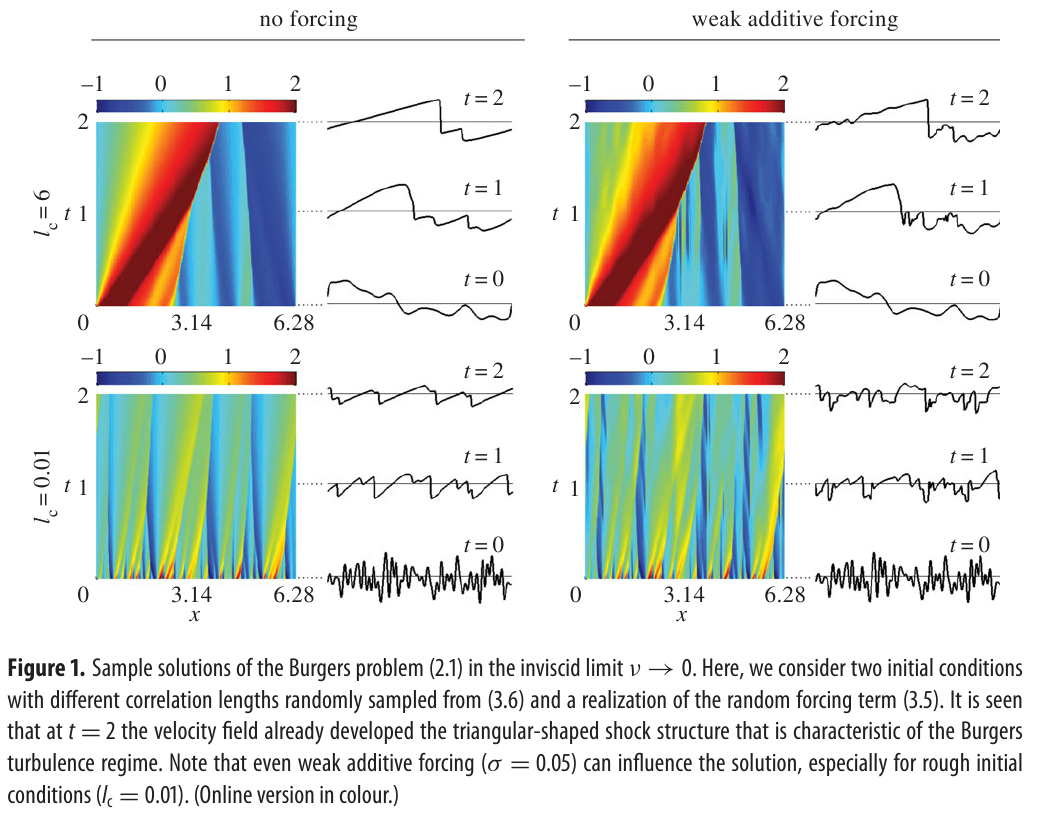
\includegraphics[width=\textwidth]{2.png} 

\end{frame}
\end{withoutheadline}
%==============================================================
\section{Assumptions}
\begin{withoutheadline}

\begin{frame} \frametitle{Assumptions}
Assumptions:
\begin{itemize}
\item For sake of simplicity, they considered just 1D Burger's equation. 
\item To be able to find an analytical answer, they neglect the diffusion effect, so it can be thought of a formulation for inviscid flow.
\item They assumed that the initial condition and source term are square integrable  random fields. (previouse picture shows their effect on the problem).

\end{itemize}

\end{frame}
\end{withoutheadline}
%==============================================================
\begin{withoutheadline}

\begin{frame} \frametitle{Assumptions Cont.}
\begin{itemize}
\item They further consider $f$ as a smooth noise.
\item Under these assumptions one can write $f(x, t;\omega$) and $u_0(x;\omega)$ in terms of series expansions involving proper sets of random variables.

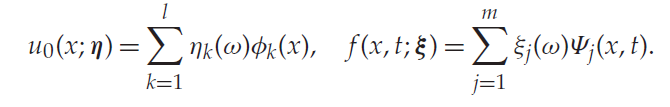
\includegraphics[width=.7\textwidth]{4.png} \\
And then the solution can be written in form of:
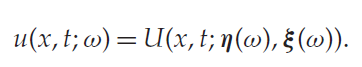
\includegraphics[width=.5\textwidth]{5.png} 
\end{itemize}

\end{frame}
\end{withoutheadline}
%==============================================================
\section{Approach}
\begin{withoutheadline}

\begin{frame} \frametitle{Approach}

\begin{itemize}
\item They use the modeling of probability density function(pdf) itself in the deterministic sens.
\item They use the Mori–Zwanzig (MZ) formalism which relies on deriving
reduced-order kinetic equations for the stochastic velocity field in the limits of small viscosity and small perturbations.
\item They combine this approach with the adaptive discontinuous Galerkin (DG)

\end{itemize}

\end{frame}
\end{withoutheadline}
%==============================================================
\section{Solution}
\begin{withoutheadline}

\begin{frame} \frametitle{Toward pdf}
The authors in their previous work, 
%
\includegraphics[width=\textwidth]{6.png} \\
showed that under these assumptions, Burger's equation admit the following joint pdf:\\
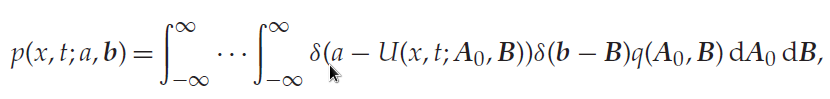
\includegraphics[width=.8\textwidth]{7.png} \\

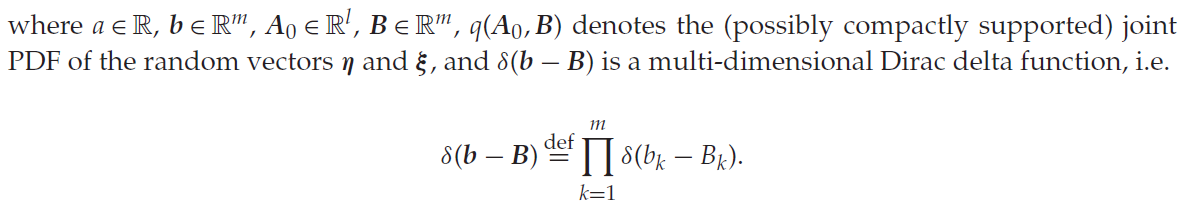
\includegraphics[width=1.08\textwidth]{8.png} 

\end{frame}
\end{withoutheadline}
%==============================================================
\begin{withoutheadline}

\begin{frame} \frametitle{Toward pdf Cont.}
Putting the above relation into the PDE results:
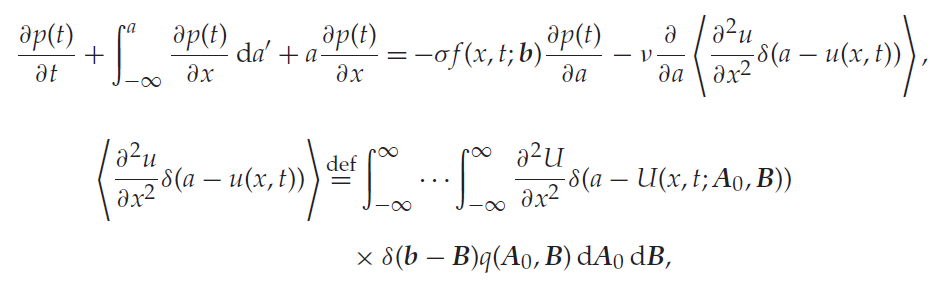
\includegraphics[width=\textwidth]{9.png} \\
Solving the above relation requires further assumptions, for more simplicity they just neglect the last term and solve it for invicsid flow.
\end{frame}
\end{withoutheadline}
%==============================================================
\begin{withoutheadline}

\begin{frame} \frametitle{Reduced-order PDF equations: Mori–Zwanzig (MZ) approach}
We can write the pde of pdf inform of:
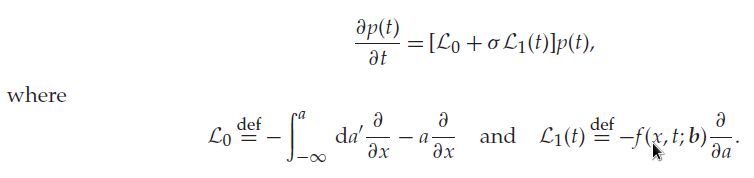
\includegraphics[width=\textwidth]{10.png} \\
by using the following transformation,\\
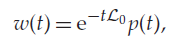
\includegraphics[width=.25\textwidth]{11.png}\\
 we can simplify it more in form of:\\
 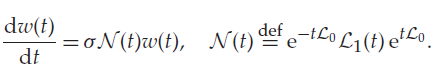
\includegraphics[width=.75\textwidth]{12.png}
\end{frame}
\end{withoutheadline}
%============================================================

\begin{withoutheadline}

\begin{frame} \frametitle{MZ approach Cont.}
\begin{itemize}
\item $\mathcal{L}_0$ depends only on the phase variable $a$, representing the velocity field, but not on the
phase variables $b$ associated with the random forcing term.

\item PDF of $u(x, t; \omega)$
can be, in principle, obtained by inverting equation  and then integrating it with respect to
$b$.

\item This operation can be conveniently represented in terms of an orthogonal projection operator.

\item So we can define the following projection ($q(b)$ denotes the joint PDF of the random vector $\xi$ appearing in the forcing term):\\
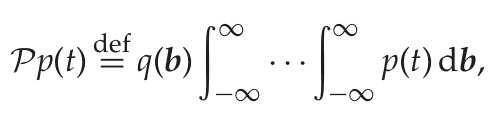
\includegraphics[width=.5\textwidth]{13.png}\\


\end{itemize}

\end{frame}
\end{withoutheadline}
%==============================================================

\begin{withoutheadline}

\begin{frame} \frametitle{MZ approach Cont.}
\begin{itemize}
\item With some simplification we can write:
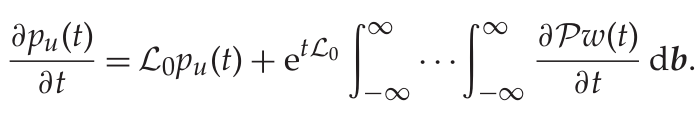
\includegraphics[width=.75\textwidth]{14.png}\\
\item Or in projected space:\\
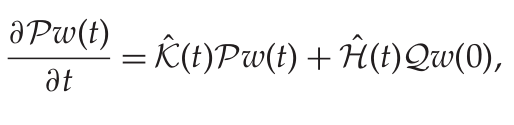
\includegraphics[width=.5\textwidth]{15.png}\\
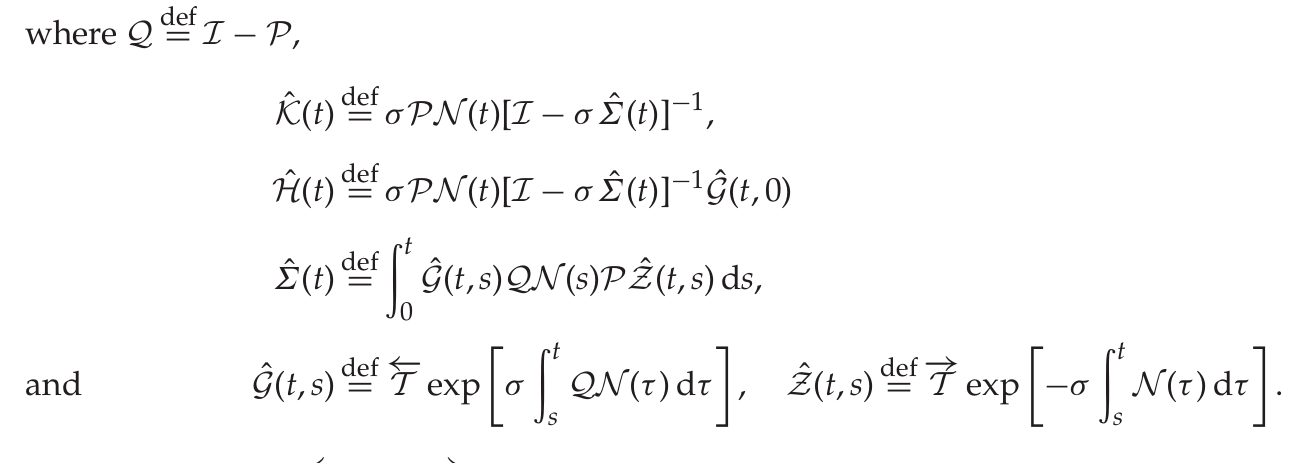
\includegraphics[width=\textwidth]{16.png}\\
\end{itemize}
\end{frame}
\end{withoutheadline}
%==============================================================
\begin{withoutheadline}
\begin{frame} \frametitle{Kinetic equations for the two-point PDF}

Almost same story can be repeated for joint distribution, but clearly more complicated:
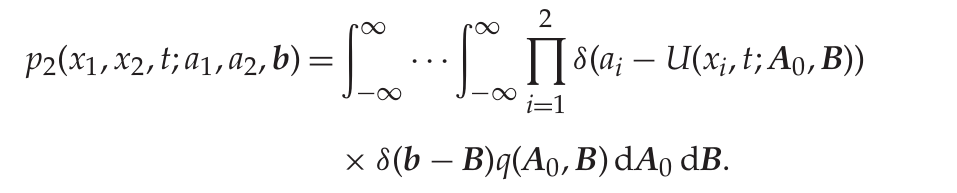
\includegraphics[width=\textwidth]{17.png}\\
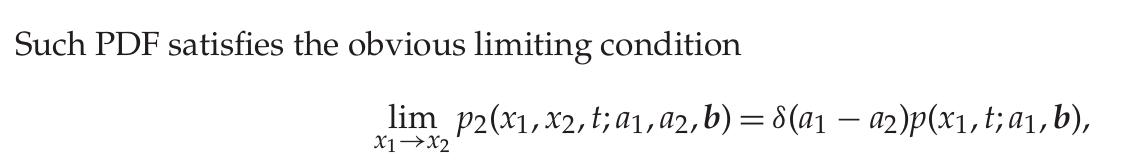
\includegraphics[width=\textwidth]{18.png}\\
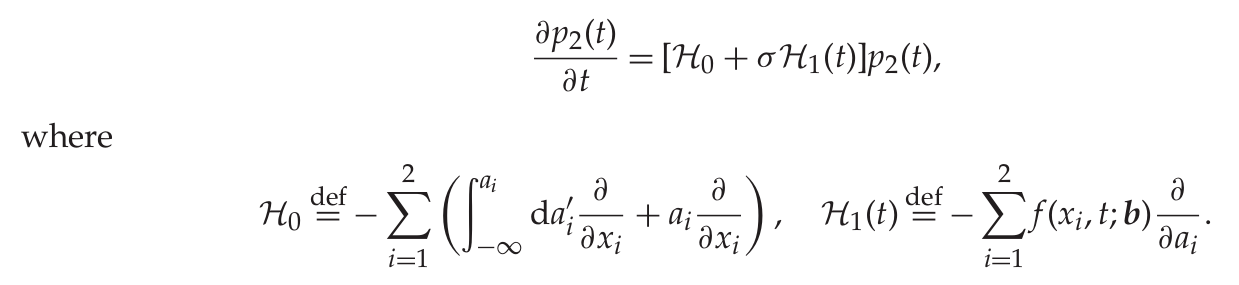
\includegraphics[width=\textwidth]{19.png}\\

\end{frame}
\end{withoutheadline}
%==============================================================
\section{Result}
\begin{withoutheadline}
\begin{frame} \frametitle{Simulation}
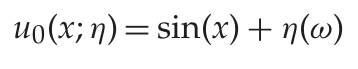
\includegraphics[width=.3\textwidth]{20.png}\\
%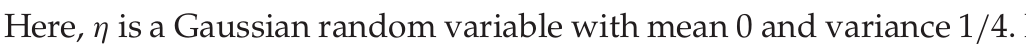
\includegraphics[width=\textwidth]{21.png}\\
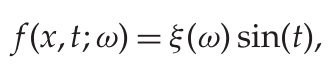
\includegraphics[width=.3\textwidth]{22.png}\\
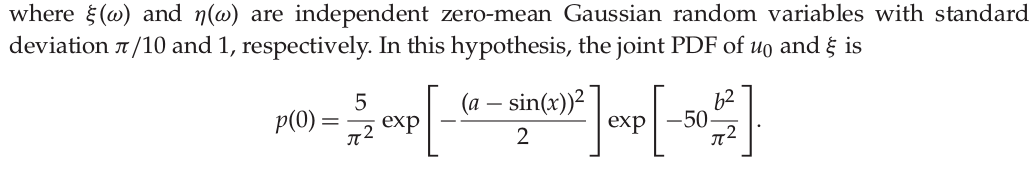
\includegraphics[width=\textwidth]{23.png}\\
\center{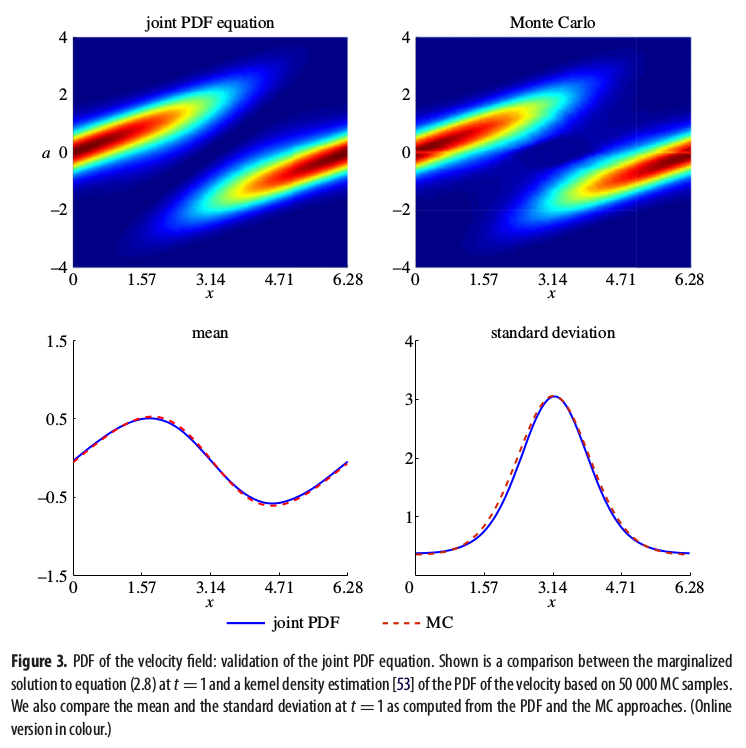
\includegraphics[width=.4\textwidth]{24.png}}\\
\end{frame}
\end{withoutheadline}
%==============================================================
\begin{withoutheadline}
\begin{frame} \frametitle{Effect of approximation}
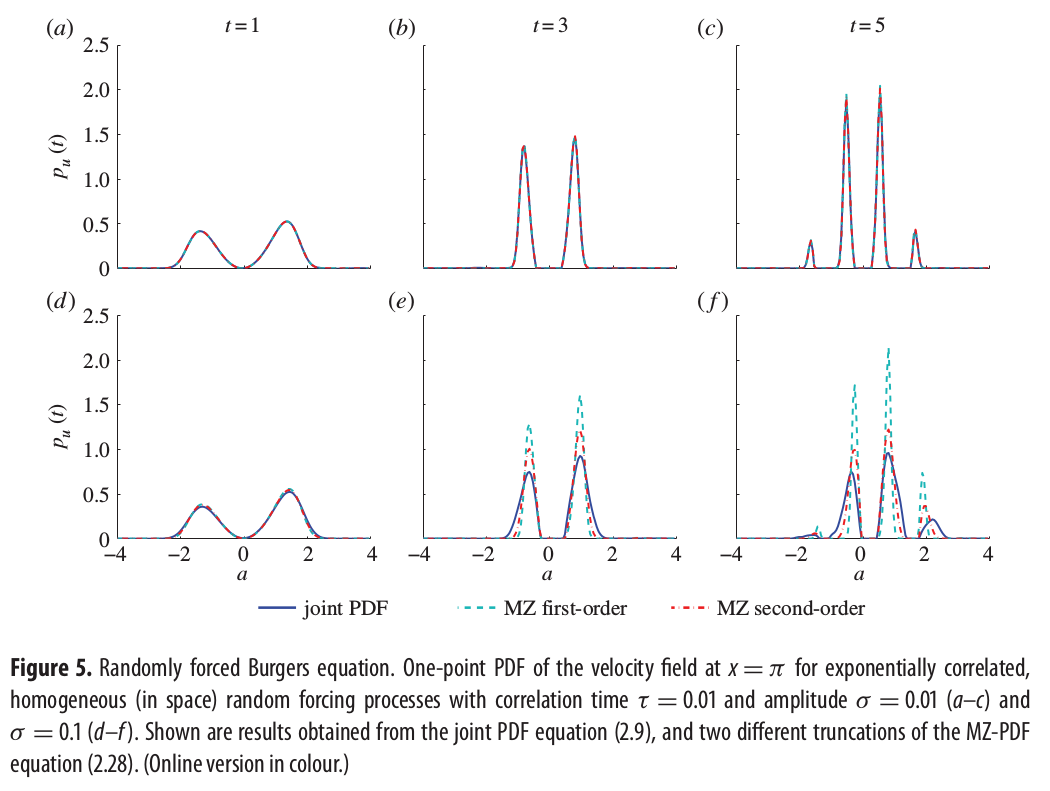
\includegraphics[width=.9\textwidth]{25.png}\\
\end{frame}
\end{withoutheadline}
%%==============================================================
%\begin{withoutheadline}
%\begin{frame} \frametitle{Kinetic equations for the two-point PDF}
%
%\end{frame}
%\end{withoutheadline}
%%==============================================================
%\begin{withoutheadline}
%\begin{frame} \frametitle{Kinetic equations for the two-point PDF}
%
%\end{frame}
%\end{withoutheadline}
%%==============================================================
%\begin{withoutheadline}
%\begin{frame} \frametitle{Kinetic equations for the two-point PDF}
%
%\end{frame}
%\end{withoutheadline}
%%==============================================================
%\begin{withoutheadline}
%\begin{frame} \frametitle{Kinetic equations for the two-point PDF}
%
%\end{frame}
%\end{withoutheadline}

\end{document}